A quick digression on the numerical computation of Fourier transforms.  It
has become all but standard to assume that when Fourier transforms of real
data are carried out in a work, the author has used the fast Fourier
transform~\cite{frigo1998fftw}~\cite{cooley1965algorithm}.  Here we
have adopted a different, much more powerful convention, which is herein briefly
described.

\subsubsection{The Fast Fourier Transform}
Recall that for a finite number of sampling points, the discrete
Fourier transform (DFT) maps a set of discrete complex input data
$x = \left\{x_1\dots x_n : x_n\in\mathbb{Z}\right\}$ onto a set of
discrete complex output data $X =
\left\{X_1\dots X_k : X_k\in\mathbb{Z}\right\}$.  This is defined by the
formula
\begin{equation}
X_k = \sum_{n=1}^{N} x_n\, \me^{\mi 2\pi k n/N}, \qquad k=1,\ldots,N
\label{eqn:dft}
\end{equation}

Direct computation of a DFT is of $O(N^2)$ complexity for $N$ sampling
points.  However, if the DFT data is linearly sampled, a fast Fourier
transform (FFT) can be used. The FFT is able to compute sums of the form of
\Equation{eqn:dft} in $O(N \log N)$ time.  The ``cost'' of this
computational efficiency is that the sampling of $X_k$ is fixed
according to the sampling of $x_n$.

\begin{figure}[ht]
\centering
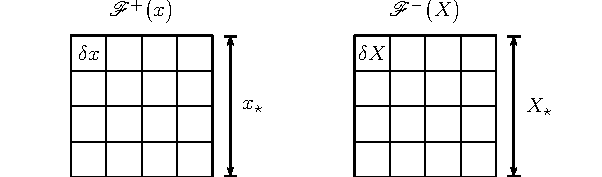
\includegraphics[keepaspectratio]{speckle/figures/fftdrawing.pdf}
\caption{Coordinates in the fast Fourier transform.}
\label{fig:fftdrawing}
\end{figure}
Because of this, there is a symmetric set of relationships for the mapping
$x_n \mapsto X_k$ (and vice versa) in the FFT.  For example, assume one
obtains $N$ samples of $x$ with bounds $x_1$ and $x_N$.  The
spacing $\delta x$ between $x_n$ and $x_{n+1}$ is just the range (denoted
by a $\star$)
$x_\star = x_N-x_1$ divided by the number of samples, $N$,
\begin{equation}
\delta x = \frac{x_\star}{N}
\end{equation}
The resultant transform in terms of $X$ has units inverse to that of $x$
\begin{equation}
\delta X = \frac{1}{x_\star}
\end{equation}
and
\begin{equation}
X_\star=\frac{1}{\delta x}=\frac{N}{x_\star}
\end{equation}
Restated, these relationships are
\begin{align}
\delta x &= \frac{x_\star}{N}\qquad x_\star
=\frac{1}{\delta X} \\
\delta X &= \frac{1}{x_\star}\qquad X_\star = \frac{1}{\delta x}
\label{eqn:fftrelationships}
\end{align}

\subsubsection{The Chirp-Z Transform}
As hinted at, there is a much more interesting way of doing things.
Consider a more general type of DFT of the form
\begin{equation}
X_k = \sum_{n=1}^{N} x_n\, z_k^n, \qquad k=1,\ldots,M
\label{eqn:czt}
\end{equation}
for $N$ elements of input $X_n$ and $M$ elements of output $x_k$ as a
function of the (sampled) complex variable  $z_k$.  This is called the
chirp-z transform~\cite{rabiner1969chirp}~\cite{rabiner1969chirp2}.
If we define
\begin{equation}
z_k = \me^{\mi 2\pi k/N}, \qquad k=1,\ldots,N
\end{equation}
we recover \Equation{eqn:dft}.  Note that the size of $x_n$ and $X_k$
are not the same.  Let us now generalize $z_k$ to a contour in the complex plane
\begin{equation}
z_k = A W^k, \qquad k=1,\ldots,N
\end{equation}
where $A$ and $W$ are complex numbers.  Specifically, $A$ defines the
starting point and $W$ the complex ratio between adjacent points on the
contour.  For $M=N$, $A=1$ and $W=\exp(\mi 2 \pi/N)$, \Equation{eqn:dft}
is again recovered.  

The amazing property here is that we can choose resolution and coordinates
of the output field.  For example, suppose one samples $x$ with $N$ samples
of spacing $\delta x$.  If we want to obtain $M$ samples in the output
$X$ field with spacing $\delta X$ beginning with $X_1$, we set
\begin{align}
								W&=\exp(\mi 2 \pi \delta x \delta X)\\
								A&=\exp(\mi 2 \pi X_1 \delta x)
\end{align}

Remarkably, the chirp-z transform can be computed with the same efficiency
as the FFT.  Consider the relationship
\begin{equation}
n k = \frac{-(k-n)^2}{2} + \frac{n^2}{2} + \frac{k^2}{2}
\end{equation}
Using this, \Equation{eqn:dft} can be rewritten
\begin{align}
								X_k &= \sum_{n=1}^{N} x_n\, \me^{\mi 2\pi k n/N} \qquad k=1,\ldots,N\\
								X_k &= \me^{\mi \pi k^2/N} \sum_{n=1}^{N} \left(x_n\, \me^{\mi \pi n^2/N}\right)\,
								\me^{\mi \pi(k-n)^2/N}\qquad k=1,\ldots,N\\
\end{align}
which is simply a convolution.  Because of the convolution theorem, which
states that the Fourier transform of the
convolution of two functions $f$ and $g$ is simply the product of the
Fourier transforms of $f$ and $g$, namely
\begin{equation}
\ff{\left(f \star g\right)} = \ff{x}\ff{g}
\end{equation}
the chirp-z transform can be expressed as a pair of FFTs, and thus be
efficiently computed.
%which is simply a convolution of $a$ and $b$, where
%\begin{align}
%a_n &= x_n\, \me^{\mi \pi n^2/N}\\
%b_n &= \me^{\mi \pi(k-n)^2/N}
%\end{align}
